\documentclass[10pt,twocolumn,letterpaper]{article}

\usepackage{cvpr}
\usepackage{times}
\usepackage{epsfig}
\usepackage{graphicx}
\usepackage{amsmath}
\usepackage{amssymb}
\usepackage{subcaption} 
\usepackage{float}
\usepackage[boxed]{algorithm2e}
\usepackage{algorithmic}
\usepackage{color}
\definecolor{darkred}{rgb}{0.8,0,0}
\definecolor{darkgreen}{rgb}{0,0.6,0}
\definecolor{darkblue}{rgb}{0,0,0.6}

% Include other packages here, before hyperref.

% If you comment hyperref and then uncomment it, you should delete
% egpaper.aux before re-running latex.  (Or just hit 'q' on the first latex
% run, let it finish, and you should be clear).
\usepackage[pagebackref=true,breaklinks=true,letterpaper=true,colorlinks,bookmarks=false]{hyperref}

% TODO: Uncomment this line to enable the RULER, which I think we need for the final submission? Verify this.
\cvprfinalcopy % *** Uncomment this line for the final submission

\def\cvprPaperID{****} % *** Enter the CVPR Paper ID here
\def\httilde{\mbox{\tt\raisebox{-.5ex}{\symbol{126}}}}

% Pages are numbered in submission mode, and unnumbered in camera-ready
% \ifcvprfinal\pagestyle{empty}\fi
\begin{document}

%%%%%%%%% TITLE
\title{RetroGAN: Translating Unpaired Video Game Images Using CycleGANs}

\author{Andrew Rollings, Michael Townsend, Tyler Thurston\\
Georgia Institute of Technology\\
% NOTE: Do we include email?
{\tt\small arollings3@gatech.edu, mtownsend31@gatech.edu, tthurston7@gatech.edu}
}
% For a paper whose authors are all at the same institution,
% omit the following lines up until the closing ``}''.
% Additional authors and addresses can be added with ``\and'',
% just like the second author.
% To save space, use either the email address or home page, not both

\maketitle
%\thispagestyle{empty}

%%%%%%%%% ABSTRACT
\begin{abstract}
   Video games from the retro era have a signature style due to the 8-bit and 16-bit technology at the time. Limitations on resolution, color, bandwidth, and processing power all created constraints that limited the vision and scope of what video game creators could implement. Using a CycleGAN architecture to allow unpaired translation, we can learn from screenshot data of two separate video game generations (8-bit and 16-bit) and translate images from one generation to the other. Our results show that we can take images from the Nintendo Entertainment System (NES) and Super Nintendo (SNES) and translate screenshots from both consoles into the style of the other. Experiments demonstrate that the CycleGAN architecture can learn many constraints of each system in order to perform relatively accurate translations between generations.
\end{abstract}

%%%%%%%%% BODY TEXT
\section{Introduction/Background/Motivation}
%\textit{\textcolor{blue}{(5 points) What did you try to do? What problem did you try to solve? Articulate your objectives using absolutely no jargon.}}

In the 1980s, 8-bit consoles were king. These were characterized by limited color palettes and relatively simple 2D graphics. In the 1990s, 16-bit consoles took over and offered increased power, color palettes and the ability to display more complex graphics.\\
Despite huge advances in technology, retro-games from the 8- and 16-bit eras remain popular, as evidenced by the number of remakes, emulators, modern ``Indie'' games using pixel art and even specialist magazines dedicating to retro gaming.\\
Our experiment is based on the observation that the primary difference between 8- and 16-bit games (as exemplified by the NES and SNES, respectively) was in the fidelity of the graphics. Additionally, many of the graphical remasters today view the 16-bit era as the gold standard in pixel-based artwork, given that the graphical capabilities of the SNES still allowed artists to express themselves far more than the limited NES.\\
Our primary objective is to train two systems, one that can take in an 8-bit NES graphic and ``up-convert'' it to a realistic 16-bit version and another system that can take in a 16-bit SNES graphic and ``down-convert'' it to a realistic 8-bit version.

%\textit{\textcolor{blue}{(5 points) How is it done today, and what are the limits of current practice?}}

Another area of interest is in software emulators that are often used to breathe life into older games. For example, the Nintendo Switch provides a paid emulation service that allows players to access a library of older games. In some cases, the emulators provide graphical filters that allow the appearance of the game to be altered (e.g. a CRT filter, or a resolution up-scaling filter). However, currently the only way to improve the graphical color depth of a game is for artists to redraw all of the game's graphics.

%\textit{\textcolor{blue}{(5 points) Who cares? If you are successful, what difference will it make?}}

If successful, this can allow the graphical content of a particular video game console to be translated into the style of another. Pixel artists are in very high demand and creating high quality pixel art is one of the largest financial strains that can be put on games, and is very time consuming/labor intensive. Pixel artists are often so hard to find that studios will save money by switching to 3D modeling as there are more artists and tools to assist them. This could allow for pixel artists to become more efficient, taking images from a previous game or console generation and translating it to the current project's generation. For instance, if one wished to modernize an 8-bit game, retroGAN enables someone to take the images from the original game and create new baseline screenshots for the sequel. Pixel artists would only need to tweak the translation instead of starting from scratch. There is also the interesting possibility of creating a real-time filter that could do this conversion ``on-the-fly'' as the game is being played. Additionally, this conversion process is not constrained to translation between NES and SNES, and could be done on other consoles and generations given suitable datasets.

%\textit{\textcolor{blue}{(5 points) What data did you use? Provide details about your data, specifically choose the most important aspects of your data mentioned \href{https://arxiv.org/abs/1803.09010}{here}. You don’t have to choose all of them, just the most relevant.}}

Datasets for NES/SNES images did not exist in a suitable form, so we created our own from various screenshot databases on the internet. We implemented our own pre-processing, which included unsupervised color clustering to remove image artifacts, clamping colors to more closely adhere to the console's original color palette, resizing and cropping as appropriate, and other noise reduction techniques. This provided us with a reasonably large set of images that were organized into quality bands based on how much preprocessing was required. We cover this in more detail later in the paper.

%-------------------------------------------------------------------------
%------------------------------------------------------------------------
\section{Approach}

%\textit{\textcolor{blue}{(10 points) What did you do exactly? How did you solve the problem? Why did you think it would be successful? Is anything new in your approach?}}

We attempted to implement translation between video game images from different generations. The primary problem was a lack of paired image data (an image from each generation) since each console generation consists almost solely of different games (with a small number of remakes). We thought CycleGAN had the potential to be a solution as it doesn't require paired data due to the cyclic process for training. That is, a NES image can be converted to a SNES fake by one leg of the cycle, and then the SNES fake can be converted back to a NES ``fake fake'' by the reverse leg. Then the round-trip images (the NES original and its doubly-converted ``fake fake'') can be compared for differences. In an ideal system, the real image and the ``fake fake'' image would be virtually identical. Both directions of the conversion process (NES$\rightarrow$SNES and SNES$\rightarrow$NES) can be cross-checked in this fashion.

We initially started by taking the driver code\footnote{https://github.com/junyanz/pytorch-CycleGAN-and-pix2pix, Commit Id 00d5574908eb66fe0127b32d7b030001453f21d0} for the original CycleGAN paper \cite{CycleGAN}, implemented in Python with PyTorch. We then removed all of the code not directly related to the CycleGAN model and added our own datasets, pre-processing, augmentation, hyper-parameter tuning code, and metrics. Our code can be viewed at \url{https://github.com/team-triforce/retroGAN}.

Given the almost miraculous results in the literature that have been achieved using CycleGANs with unpaired datasets (and admittedly vast computing resources way beyond our reach), we were reasonably confident that we could use similar techniques to perform a non-trivial conversion between 8-bit and 16-bit screenshots of games. We expected the 16$\rightarrow$8-bit conversion to be much simpler than the 8$\rightarrow$16-bit conversion, but we were hopeful that we might be able to achieve at least some worthwhile results in the latter case.

While the CycleGAN architecture has been used to solve many problems, our dataset is unique and to our knowledge, no other work has properly explored unpaired image-to-image translation in this domain.

%\textit{\textcolor{blue}{(5 points) What problems did you anticipate? What problems did you encounter? Did the very first thing you tried work?}}

The main problem we expected was a lack of clean data. While there are plenty of screenshots of games available across the Internet, we could not find any pre-sorted collections of clean images. As such, we ended up writing several custom web scrapers and image processing tools to collect and homogenize screenshots from several game catalog websites. This process is covered in more detail later in the paper.

Additionally, we had concerns if CycleGAN would be able capture the ``pixel-perfect'' constraints and requirements for the conversion process. Previously, CycleGANs have been typically used for experiments that have not required such exact results; for example, the well-known Horse to Zebra results were not conditioned on the exact shades of white and black of the zebra stripes.

Conversely, in our situation, there are several palette restrictions that apply to the NES and SNES consoles. While the main difference between these consoles is their available color palettes, the NES also has several other graphical restrictions that place some difficultly in quantifying restrictions on the number of colors in a particular areas of the screen. The SNES also has similar restrictions, although nowhere near as severe. This was anticipated to be very difficult to generalize without magnitudes more data then we had available to us (approximately 100,000 images of varying quality between the two consoles). We didn't see great results in our first attempt, however after performing some additional pre-processing (covered later in this paper), we started seeing interesting results with convincing translations very early on.

%\textbf{\textcolor{blue}{Important: Mention any code repositories (with citations) or other sources that you used, and specifically what changes you made to them for your project.}}

\subsection{NES / SNES Palette Considerations}
The NES palette comprises 56 fixed colors\footnote{https://en.wikipedia.org/wiki/List\_of\_video\_game\_console\_palettes}, whereas the SNES is more flexible with a full 15-bit RGB palette (with 5 bits for each of the red, green and blue channels)\footnote{https://en.wikipedia.org/wiki/List\_of\_monochrome\_and\_RGB\_color\_formats}, as shown in Figures \ref{fig:nes} and \ref{fig:snes} respectively.

As previously mentioned, there are some additional restrictions to how these colors can be used, but we do not cover them here; they are of more concern to emulator writers, and it was hoped that \--- given enough data \--- the CycleGAN would be able to figure these out for itself.

As such, for an effective conversion, the GAN must learn to conform to each palette. In the case of SNES${\rightarrow}$NES, this could be as simple as a naive nearest color reduction from the 15-bit SNES palette to the fixed NES palette. Similarly, for the NES${\rightarrow}$SNES conversion, the GAN could simply ensure that the chosen colors fit the 15-bit RGB restriction. However, we hoped for (and observed) more complex behaviors than this, implying that the GAN was able to somewhat successfully extract more of the stylistic differences between NES and SNES graphics. This will be discussed in later sections.

\begin{figure}[htp]
   \centering
   \begin{subfigure}[b]{0.235\textwidth}
      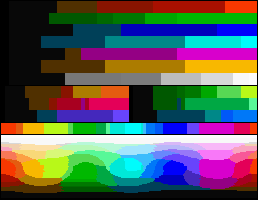
\includegraphics[width=\textwidth]{figures/NES_palette_color_test_chart.png}
      \caption{NES 56 Color Palette}
      \label{fig:nes}
   \end{subfigure}
   \begin{subfigure}[b]{0.235\textwidth}
      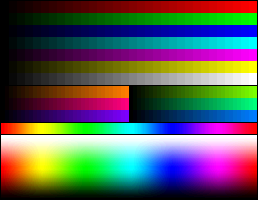
\includegraphics[width=\textwidth]{figures/SNES_palette_color_test_chart.png}
      \caption{SNES 15-bit Palette}
      \label{fig:snes}
   \end{subfigure}
   \caption{Color palettes for NES and SNES}
\end{figure}

\subsection{Generative Models and CycleGANs}
For our main architecture, we chose CycleGAN for the many positives it brings. First, being a Generative Model, it brings us the ability to generate new models via sampling from our implicit density estimation. On top of that, we also were drawn by the advantages of specifically Generative Adversarial Networks(GANs)\cite{GAN}. GANs provide several benefits over other generative models, including not needing labeled data as GANs are unsupervised. They are also flexible on the types of data they ingest. Most importantly, since they sample from their density instead of doing any kind of averaging, GANs result in the sharpest images over other generative models. This is a very important property as retro graphics involve small, sharp pixel placement which makes this a vital quality for this dataset.

Finally, we chose CycleGAN\cite{CycleGAN}, as it provides the ability to translate between two datasets without the need for paired images. Instead of the usual GAN architecture of a single generator and discriminator, the CycleGAN architecture uses mappings: $G$ and $F$ with the goal of having $G$ learn a mapping from domain $X \rightarrow Y$ such that $G(X)$ is indistinguishable from the distribution $Y$ using adversarial loss. However, due to the low constraints of unpaired data, a second, inverse mapping $F: Y \rightarrow X$ is created to induce a cycle consistency loss to push $F(G(X)) \approx X$, as shown:
\begin{equation*}
   G: X \rightarrow Y, F: Y \rightarrow X : F(G(X)) \approx X
\end{equation*}

These mappings are combined with two \textit{cycle consistency losses} that can capture the intuition that translating from one domain to another and back again should result to something similar to the original input.

Additionally, an \textit{identity loss} is used to provide color/hue stability. This is defined as $F(X) \approx X$ and $G(Y) \approx Y$. The \textit{identity loss} is combined with the \textit{cycle consistency loss} proportionally as determined by a bias hyperparameter.


\begin{figure}[H]
   \centering
   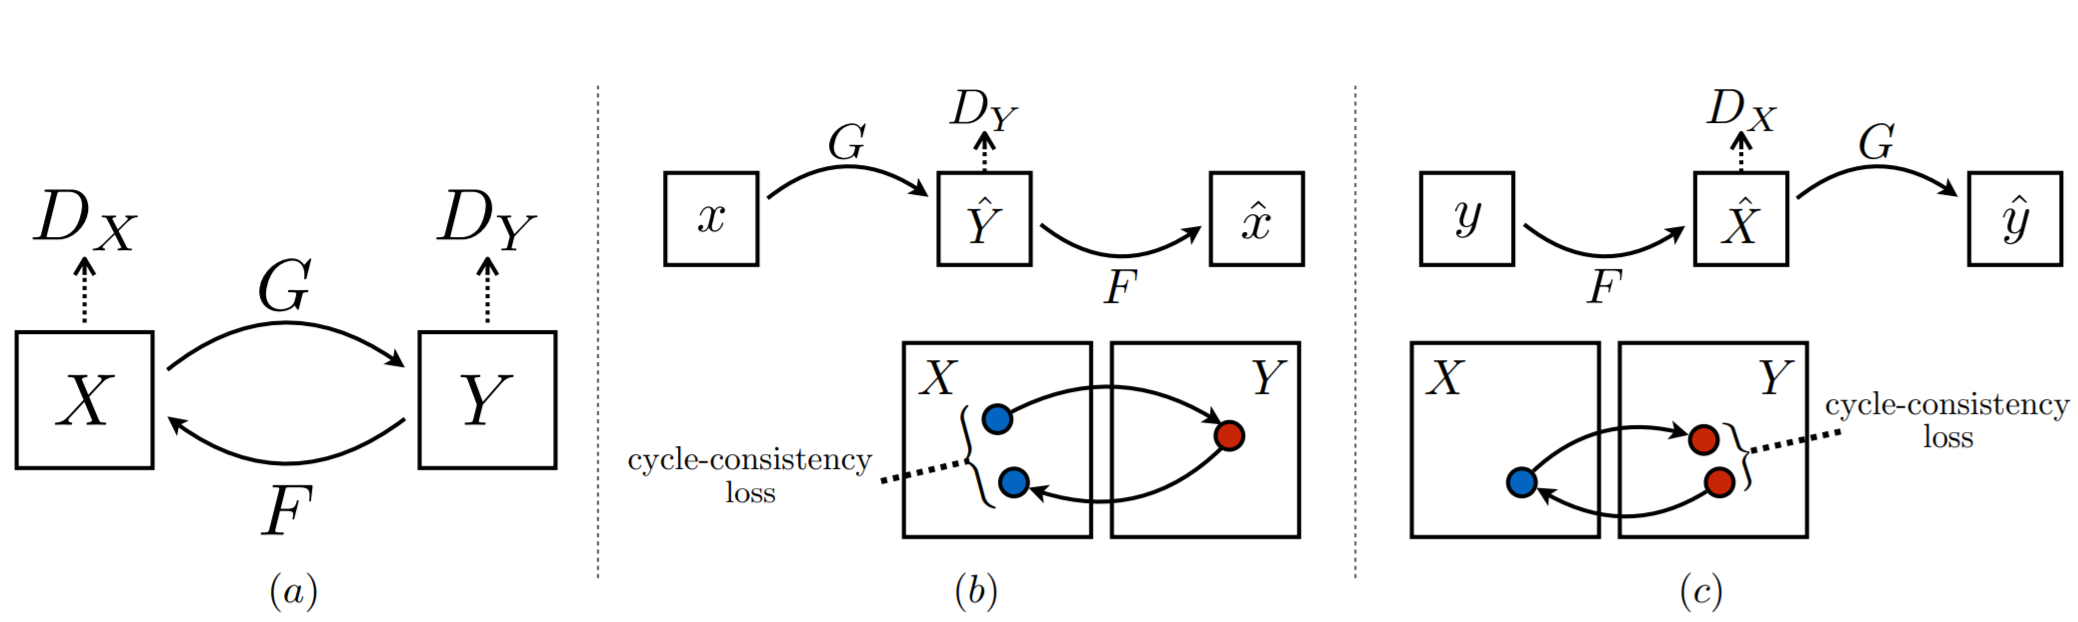
\includegraphics[width=0.485\textwidth]{figures/CycleGANChart.png}
   \caption{CycleGAN Architecture}
\end{figure}


\section{Experiments and Results}

%\textit{\textcolor{blue}{(10 points) How did you measure success?}}

The CycleGAN framework allowed for significant configurability of hyperparameters, and we took full advantage of the flexibility provided. As such, for our first pass success measure, we selected for the hyperparameters that showed the smallest amount of loss for at least \textit{one} direction of the cycle. This gave us a shortlist of candidates to examine that we evaluated manually to determine which to investigate further. One interesting (but not entirely unexpected) observation we found was that the cycle performance was not even; a set of hyperparameters that performed well for the NES$\rightarrow$SNES conversion would not necessarily perform well for the SNES$\rightarrow$NES conversion, and vice versa.

For each promising candidate set, we then ran a customized metric to evaluate the final images for their adherence to the hardware restrictions of each console. We produced several iterations of this metric, before finally settling on Algorithm \ref{alg:alg1}. This was applied as a post-training evaluation metric and was not a learned parameter.

This metric scores an image based on how closely the pixels match the target console palette modulated by the percentage of image pixels that match the target palette exactly. This modulation was necessary to compensate for the fact that the SNES palette has many more entries, and consequently, it was easier for the algorithm to score highly as any selected color was never too far away from a valid palette entry in RGB space. A perfect metric of either system would require accounting for hundreds of variables(pixel limit, per-pixel color palette limits, transparency limitations, max sprites per screen, etc), however this would be a task outside the scope of this paper and would heavily depend on domain knowledge, so we chose a metric that focuses on color palette, as it's a much more tractable task and is a metric that could be adapted to consoles other than just the NES/SNES.

In practice, we found that using the stricter NES metric produced more meaningful results; that is, for the SNES$\rightarrow$NES conversion, we found that measuring the increase in value for this metric between the real SNES and fake NES image was a strong indicator of success. Conversely, for the NES$\rightarrow$SNES conversion, the decrease in value of this metric was a good indicator of success.

%\textit{\textcolor{blue}{What experiments were used?}}

Using the hyperparameter search driver, each of the three authors ran a random hyperparameter search using the time available; once this was complete we first compared our results by the metric described above, selecting a shortlist of best candidates. We considered each direction of the cycle separately for the reasons mentioned previously. For each candidate, we performed a visual inspection of the output and reached a consensus on which of these had generated the best overall results. The final candidate from each cycle direction was then used to generate the images and graphs in the following sections.

%\textit{\textcolor{blue}{What were the results, both quantitative and qualitative? Did you succeed? Did you fail? Why? Justify your reasons with arguments supported by evidence and data.}}

\subsection{SNES$\rightarrow$NES Results}

As expected, the SNES$\rightarrow$NES conversion proved to be the most effective cycle leg. For a training group size of 2500 images from the best quality band, the averaged NES metric was $0.9848$, indicating that across all of the training images, roughly 98\% of the pixels conformed to the NES palette.


We selected several of the most aesthetically pleasing conversion images, and re-ran the NES metric on both the real and fake images, as shown in table \ref{tab:nesresults}.
These results show that, while there was definite improvement, and hence learning, the network was unable to score the same metric as the training set. For a dataset size of 2500 (with a 90/10 train/test split), the averaged SNES metric was $0.6382$, indicating that across all of the training images, roughly 64\% of the pixels conformed to the NES palette. The specific dataset size was chosen due to training time constraints.

\begin{table}[H]
   \begin{center}
      \begin{tabular}{|l|c|c|}
         \hline
         Source SNES Image      & Real     & Fake     \\
         \hline\hline
         ActRaiser              & $0.0449$ & $0.5190$ \\
         Super Ghouls 'n Ghosts & $0.0171$ & $0.3330$ \\
         \hline
      \end{tabular}
   \end{center}
   \caption{SNES$\rightarrow$NES Results (NES Metric)}
   \label{tab:nesresults}
\end{table}

These results were generated using the hyperparameters shown in table \ref{tab:sneshyperparameters}. Note that only hyperparameters different than the defaults specified in the CycleGAN code are shown. 


\begin{table}[H]
   \begin{center}
      \begin{tabular}{|l|c|}
         \hline
         \textbf{Hyperparameter} & \textbf{Value} \\
         \hline\hline
         Batch size     & $4$ \\ 
         \hline
                  GAN Mode     & lsgan\\
         \hline
         netG       & unet\_128  \\ 
         \hline
         Pre-process     & pixel double and crop \\
         \hline
         Epochs     & 50 \\
         \hline
         Decay Epochs    & 10 \\
         \hline         
      \end{tabular}
   \end{center}
   \caption{SNES$\rightarrow$NES Hyperparameters}
   \label{tab:neshyperparameters}
\end{table}

\begin{figure}[H]
   \centering
   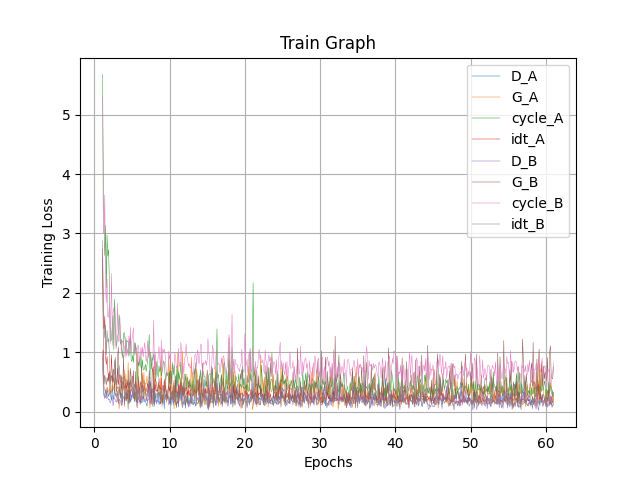
\includegraphics[width=0.475\textwidth]{figures/graphs/train_graph_nes.png}
   \caption{Training Graph with best SNES$\rightarrow$NES results}
   \label{fig:nesgraph}
\end{figure}

The generator network used a U-Net 128 architecture internally, and the discriminator network used the default basic architecture. Figure \ref{fig:unet} shows the general structure of a U-Net architecture\footnote{Adapted from \url{https://github.com/matthias-wright/cifar10-resnet}}. The generator had $41.829 \times 10^6$ trainable parameters and the discriminator had $2.766 \times 10^6$.
The ``least squares'' loss function was used by the discriminator (as determined by the \textit{lsgan} hyperparameter choice for GAN Mode.
%  41.829

\begin{figure}[H]
   \centering
   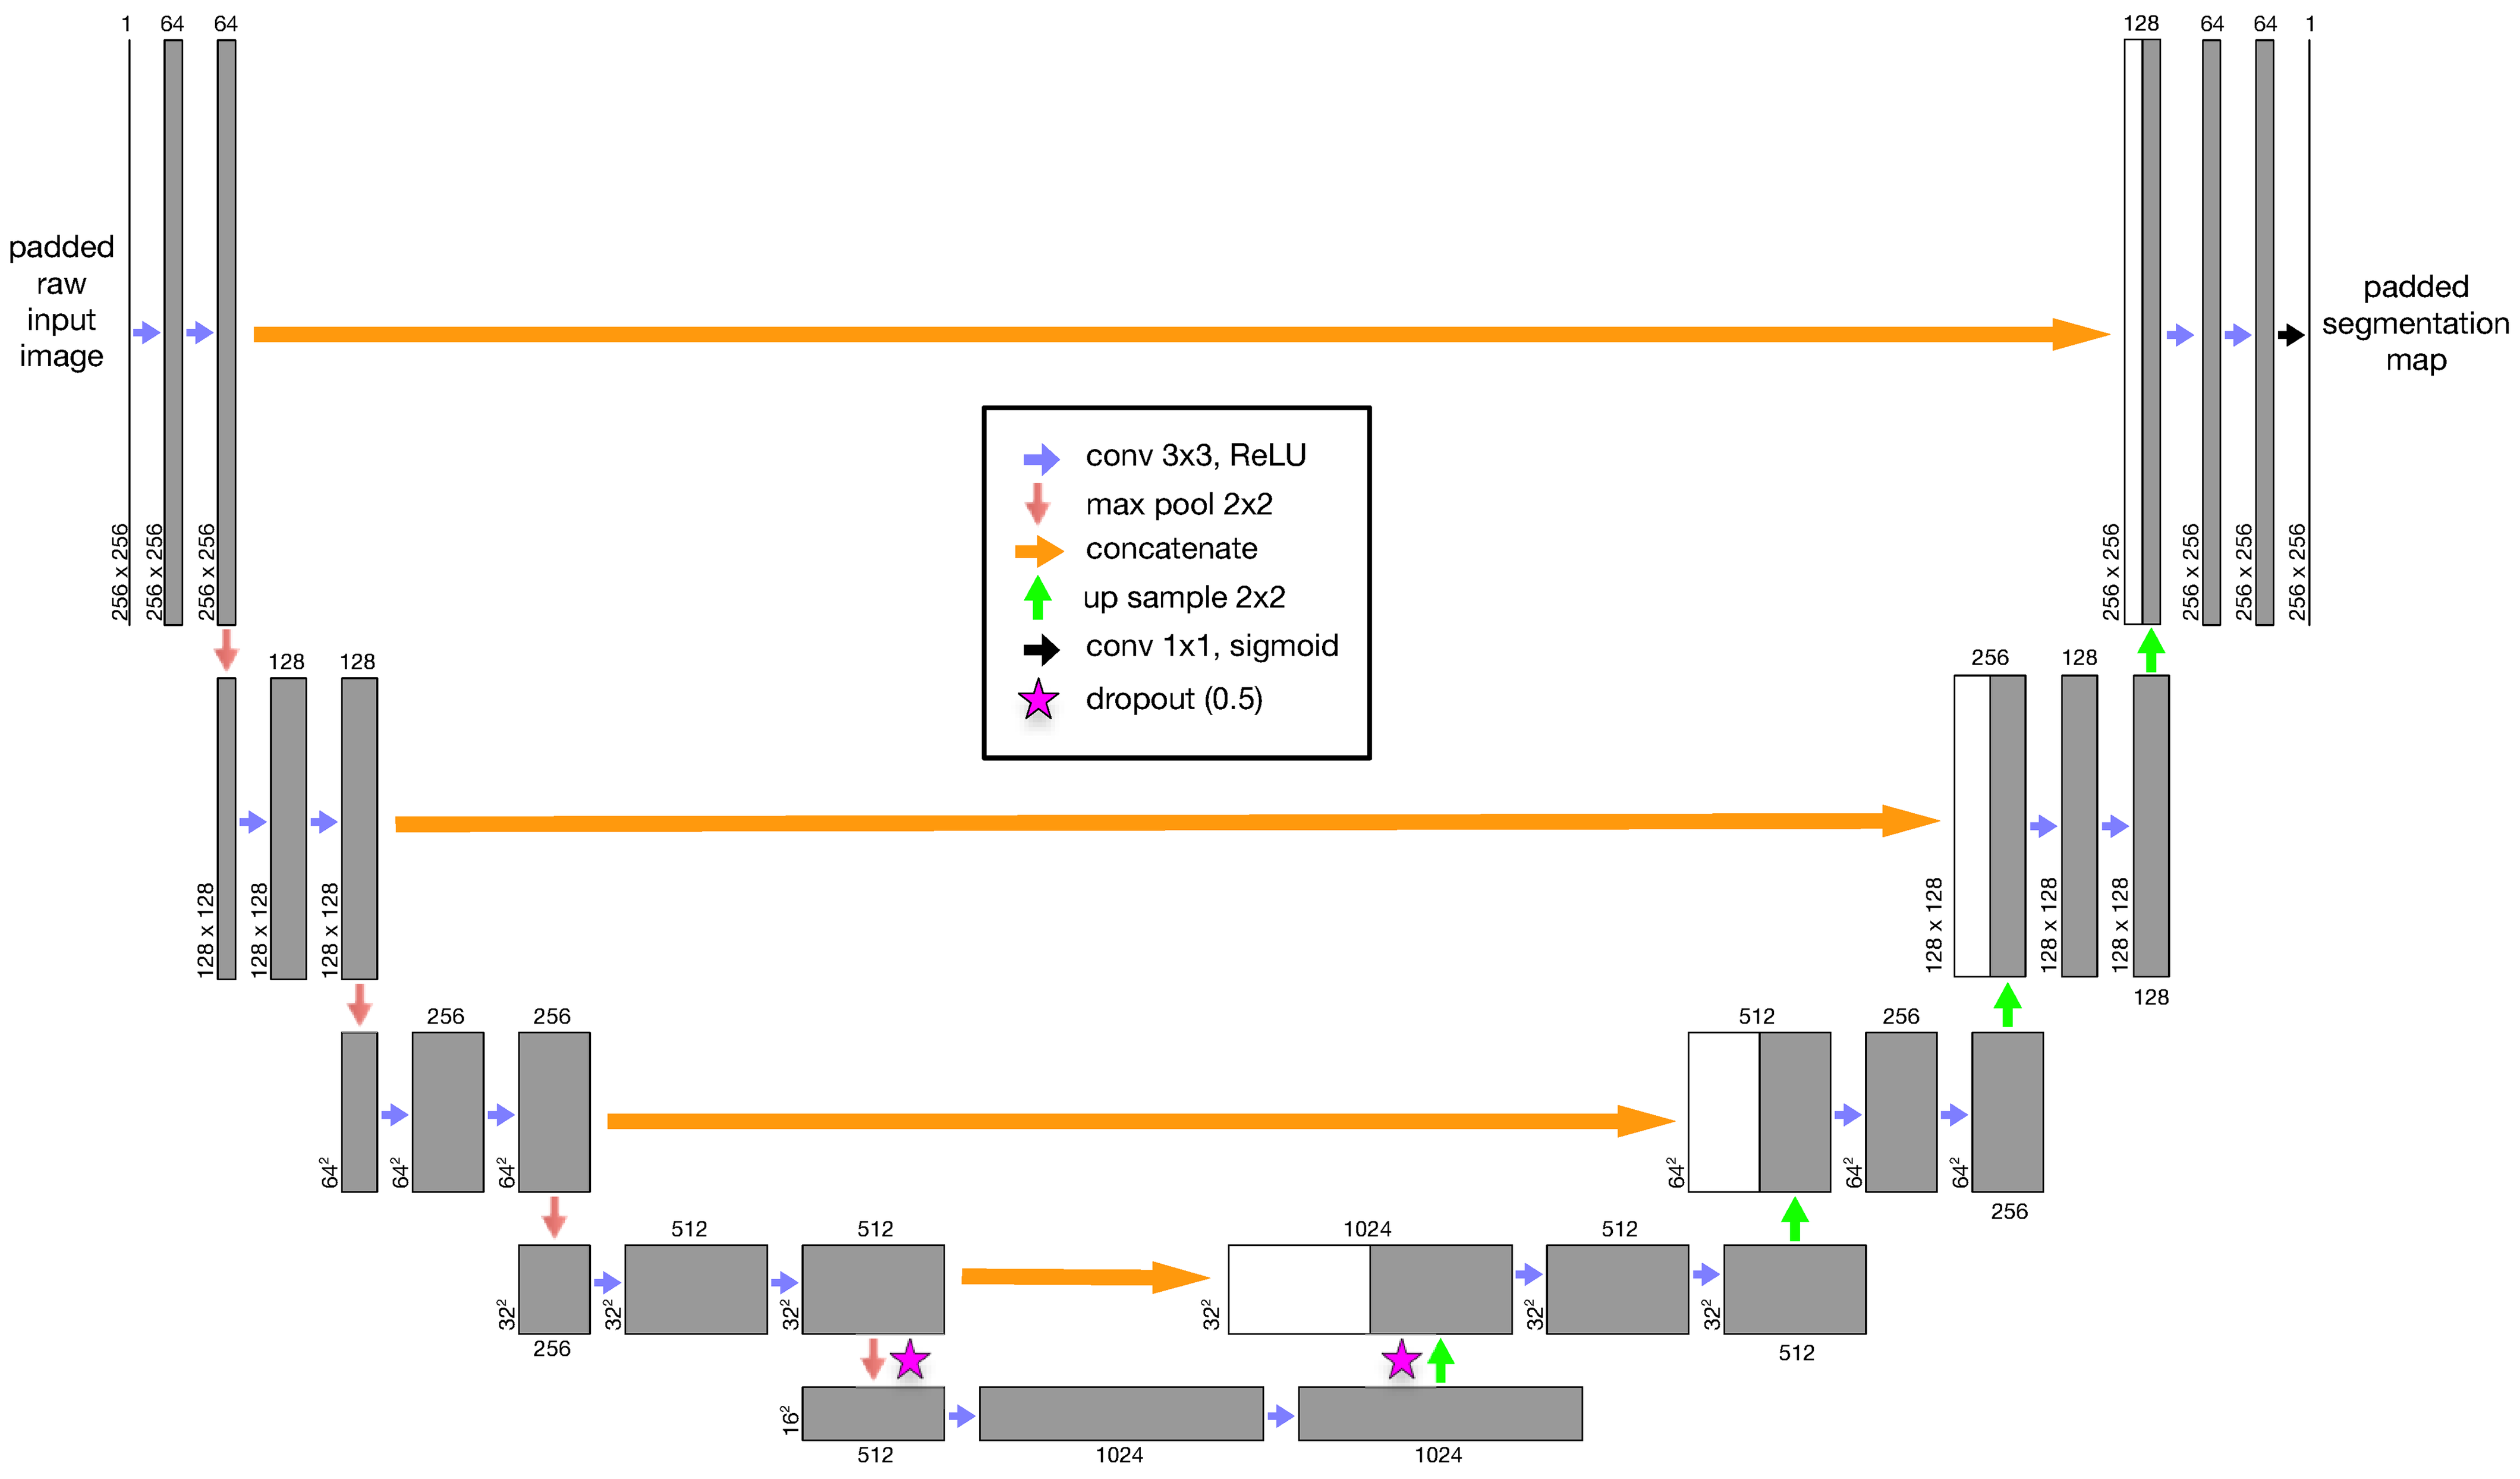
\includegraphics[width=0.485\textwidth]{figures/unet.png}
   \caption{Example U-NET Architecture}
   \label{fig:unet}
\end{figure}
% 

%% screenshot 1
\begin{figure}[H]
   \centering
   \begin{subfigure}[b]{0.225\textwidth}
      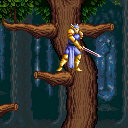
\includegraphics[width=\textwidth]{figures/snes_to_nes/AV_Mahjong_Club_(J)_(Unl)_copy__ucc__8_real_B.png}
      \caption{Real SNES Screenshot}
      \label{fig:ss1a}
   \end{subfigure}
   \begin{subfigure}[b]{0.225\textwidth}
      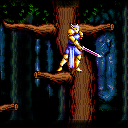
\includegraphics[width=\textwidth]{figures/snes_to_nes/AV_Mahjong_Club_(J)_(Unl)_copy__ucc__8_fake_A.png}
      \caption{Fake NES screenshot}
      \label{fig:ss1b}
   \end{subfigure}
   \caption{ActRaiser: SNES$\rightarrow$NES}
\end{figure}

%% screenshot 2
\begin{figure}[H]
   \centering
   \begin{subfigure}[b]{0.235\textwidth}
      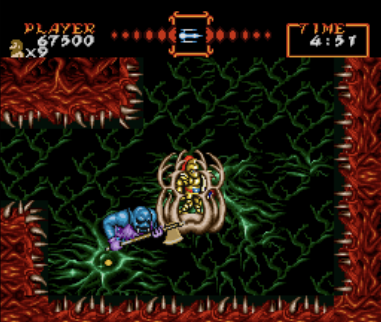
\includegraphics[width=\textwidth]{figures/snes_to_nes/ghouls_n_ghosts_real_B.png}
      \caption{Real SNES Screenshot}
      \label{fig:ss2a}
   \end{subfigure}
   \begin{subfigure}[b]{0.235\textwidth}
      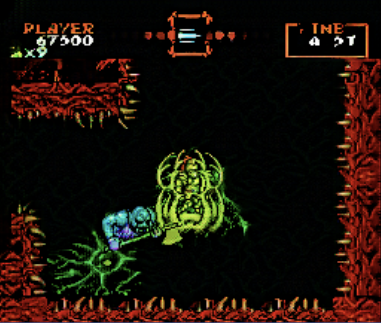
\includegraphics[width=\textwidth]{figures/snes_to_nes/ghouls_n_ghosts_fake_A.png}
      \caption{Fake NES screenshot}
      \label{fig:ss2b}
   \end{subfigure}
   \caption{Super Ghouls 'n Ghosts: SNES$\rightarrow$NES}
\end{figure}

Despite the lower metric score, a visual examination of the results in figures \ref{fig:ss1a} and \ref{fig:ss1b} show that the fake image is clearly closer to the target aesthetic, and the conversion process appears to be more involved than a simple palette conversion.
In particular, figure \ref{fig:ss1b} seems to show that different conversion criteria have been applied to different areas of the image. If one compares the lower left brighter green area in figure \ref{fig:ss2a} with the similar intensity green area just right of center, it appears that the lower left area is rendered brighter in \ref{fig:ss2b} than the right of center area, even though the same areas in the source image are of similar intensity.

Overall these results are promising, although they are far from perfect. Since we're using an imperfect metric, the fact that we chose our final network based on the performance of that metric is inducing some level of bias towards color. As we stated before, to truly represent a NES game requires accounting for many additional constraints beyond color. However, since that isn't a tractable metric we can create and our metric is centered only on color, it's reasonable that the network is prone to overfitting color at the cost of other features not reliant on color palette.

There is evidence that the network is learning beyond color though, as \ref{fig:ss2a} shows that the NES conversion removed the foggy backdrop of the original image. This is very important, as drawing a foggy background in this example was mostly likely done using transparency on the SNES, which is something that the NES can't replicate as it didn't have enough spare memory to allow for it. This is evidence that the model was able to account beyond replicating the color palette and started understanding from NES data that effects like transparency aren't possible.


\subsection{NES$\rightarrow$SNES Results}

For the NES$\rightarrow$SNES conversion we performed an almost identical analysis. We selected several of the most aesthetically pleasing conversion images, and re-ran the stricter NES metric on both the real and fake images, as shown in table \ref{tab:snesresults}.

\begin{table}[H]
   \begin{center}
      \begin{tabular}{|l|c|c|}
         \hline
         Source NES Image & Real  & Fake     \\
         \hline\hline
         Crisis Force     & $1.0$ & $0.0155$ \\
         Ninja Kid        & $1.0$ & $0.0157$ \\
         \hline
      \end{tabular}
   \end{center}
   \caption{NES$\rightarrow$SNES Results (NES Metric)}
   \label{tab:snesresults}
\end{table}

These results were generated using the hyperparameters shown in table \ref{tab:sneshyperparameters}. Note that only hyperparameters different than the defaults specified in the CycleGAN code are shown. 

\begin{table}[H]
   \begin{center}
      \begin{tabular}{|l|c|}
         \hline
         \textbf{Hyperparameter} & \textbf{Value} \\
         \hline\hline
         Batch size     & $4$ \\ 
         \hline
                  GAN Mode     & lsgan\\
         \hline
         netG       & resnet\_9  \\ 
         \hline
         Pre-process     & pixel double and crop \\
         \hline
      \end{tabular}
   \end{center}
   \caption{NES$\rightarrow$SNES Hyperparameters}
   \label{tab:sneshyperparameters}
\end{table}

\begin{figure}[H]
   \centering
   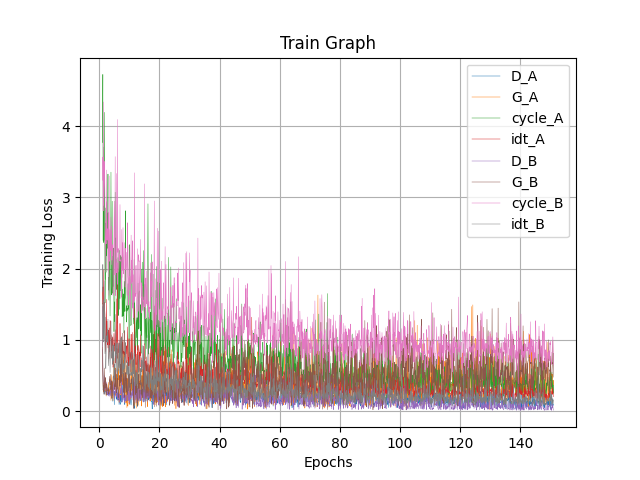
\includegraphics[width=0.475\textwidth]{figures/graphs/train_graph_snes.png}
   \caption{Training Graph with best NES$\rightarrow$SNES results.}
   \label{fig:snesgraph}
\end{figure}

The generator network used a 9-block ResNet architecture internally, and the discriminator network used the default basic architecture. Figure \ref{fig:resnet} shows the general structure of a ResNet architecture\footnote{Adapted from \url{https://github.com/matthias-wright/cifar10-resnet}}. The generator had $11.383 \times 10^6$ trainable parameters and the discriminator had $2.766 \times 10^6$.
The ``least squares'' loss function was used by the discriminator (as determined by the \textit{lsgan} hyperparameter selection for GAN Mode.
%  41.829

\begin{figure}[H]
   \centering
   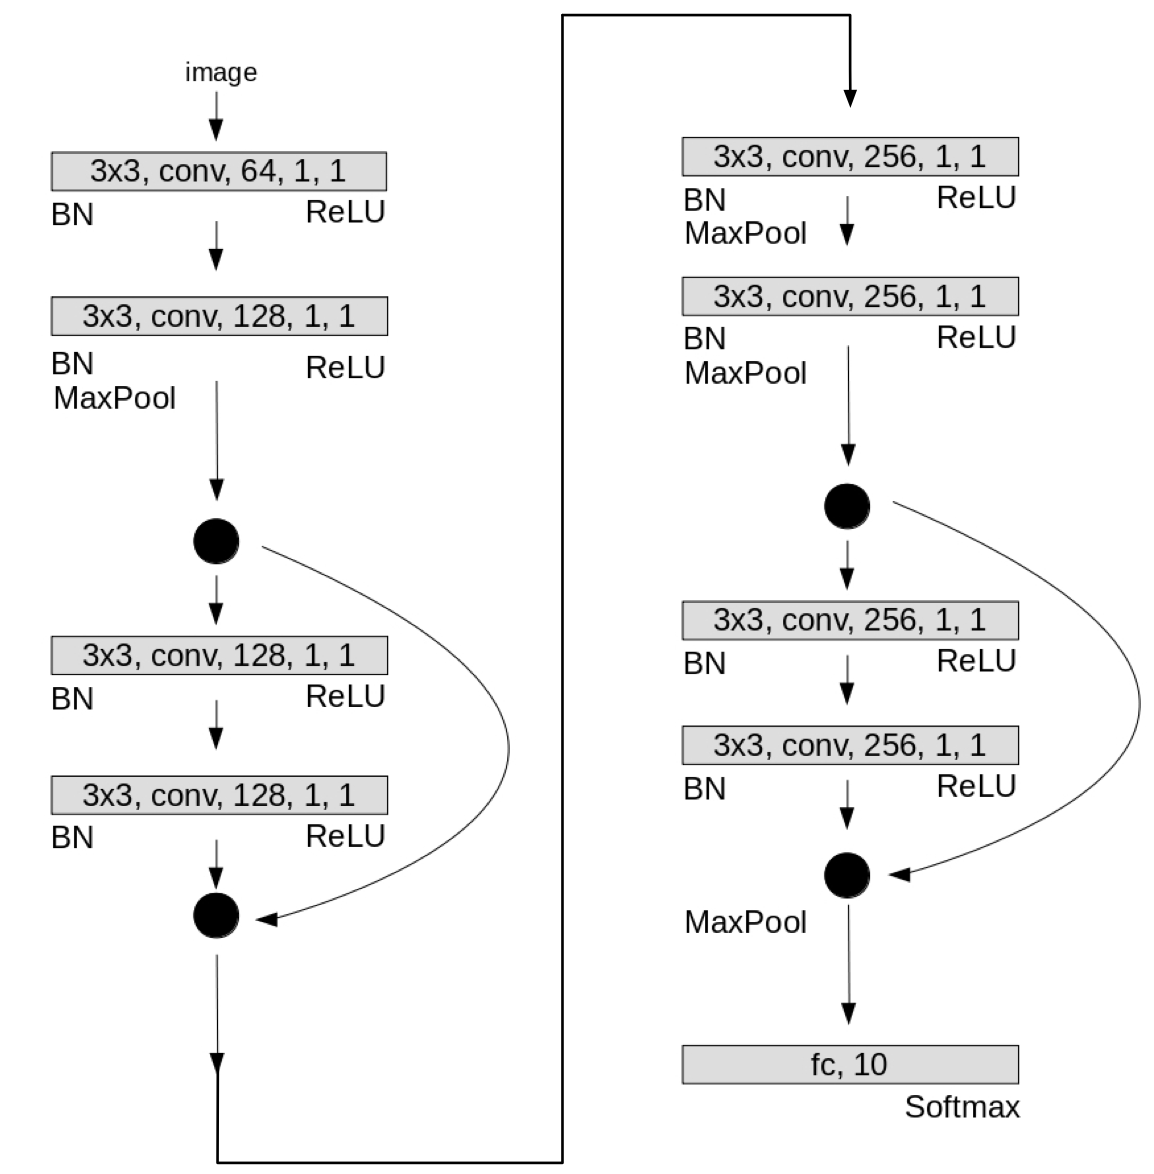
\includegraphics[width=0.475\textwidth]{figures/resnet_architecture.png}
   \caption{Example ResNet Architecture}
   \label{fig:resnet}
\end{figure}


%% screenshot 3
\begin{figure}[H]
   \centering
   \begin{subfigure}[b]{0.235\textwidth}
      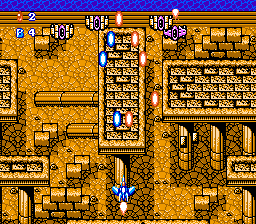
\includegraphics[width=\textwidth]{figures/nes_to_snes/Crisis_Force_(J)__ucc__12_real_A.png}
      \caption{Real NES Screenshot}
      \label{fig:ss3a}
   \end{subfigure}
   \begin{subfigure}[b]{0.235\textwidth}
      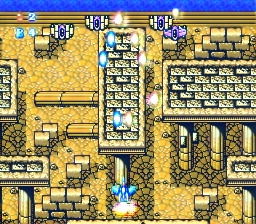
\includegraphics[width=\textwidth]{figures/nes_to_snes/Crisis_Force_(J)__ucc__12_fake_B.png}
      \caption{Fake SNES screenshot}
      \label{fig:ss3b}
   \end{subfigure}
   \caption{Crisis Force: NES$\rightarrow$SNES}
\end{figure}

%% screenshot 4
\begin{figure}[H]
   \centering
   \begin{subfigure}[b]{0.235\textwidth}
      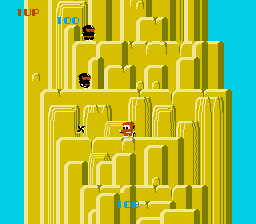
\includegraphics[width=\textwidth]{figures/nes_to_snes/Ninja_Kun_-_Majou_no_Bouken_(J)__ucc__8_real_A.png}
      \caption{Real NES Screenshot}
      \label{fig:ss4a}
   \end{subfigure}
   \begin{subfigure}[b]{0.235\textwidth}
      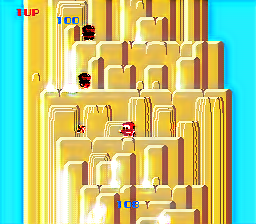
\includegraphics[width=\textwidth]{figures/nes_to_snes/Ninja_Kun_-_Majou_no_Bouken_(J)__ucc__8_fake_B.png}
      \caption{Fake SNES screenshot}
      \label{fig:ss4b}
   \end{subfigure}
   \caption{Ninja Kid: NES$\rightarrow$SNES}
\end{figure}

Although it is apparent that this leg of the conversion was not as successful as the reverse leg, it is still notable that the results show that some selective conversion has taken place. Notably, the results show that background areas tended to be lightened and blurred, bright spots tended to be blown out and made brighter, while areas of darker colors \--- particular those with black pixel outlines \--- tended to be left relatively untouched, implying that the network did at least extract some relevant feature information.

For two reasons we concluded that we underfit the model. First, the fake training images continued to improve as the training went one. At no point did the generated image's quality plateau. Second, we used smaller training sizes due to time constraints. Given more time we may have been able to use our entire dataset and fully train the model.

%%%%%%%%% CONCLUSION
\section{Conclusion And Future Work}

Our results show that despite the complications, some promising results emerged from our experiments. As expected, the results for the SNES$\rightarrow$NES conversion were better than the NES$\rightarrow$SNES due to the comparative simplicity of a down-conversion (where information loss isn't necessarily a problem) versus up-conversion, where information has to be synthesized from learned experience.

In essence, the former conversion is almost trivially easy for the CycleGAN compared to the latter.

With further experimentation and architecture tweaks, we believe that we would have been more successful with the NES$\rightarrow$SNES conversion.

Examples of possible future work could include video-based training, using pixel-perfect screen captures from console emulation software. The use of video would hopefully help the CycleGAN perform stable modifications as the game progressed. If successful, this could be used to perform real-time up-conversion of games played in an emulator.

Additional follow up work could include improvements to the scoring metrics to take into account the additional hardware restrictions, as well as the incorporation of the metrics into the respective loss functions.

Future work could also focus on expanding the consoles that the framework supports. For example, mapping from 16-bit to 32-bit or even mapping larger jumps from 16-bit to 64-bit. There would be added complexity to this, which may result in needing larger training sets or alternate loss functions.

Alternate loss functions in particular are an interesting area for further research. The CycleGAN architecture was built for the general problem on mapping images from one domain to another. However, for the specific problem of mapping images from one console generation to another, loss functions could be more precise. Others could research using the loss function to additionally model the console's graphical constraints, learning the exact color palette of each console generation.

In the short term, given more time, we would have liked to have explored the possibility of enforcing some of the palette constraints (particularly for the SNES$\rightarrow$NES conversion) by modifying the output layer of the GAN so that, for example, each pixel in the output image was represented by a one-hot encoded palette entry. This would have resulted in an output layer of size $56\times256\times256\approx3.67\times10^6$ parameters, and would have ensured palette adherence, but may well have been significantly harder to train. This implementation would not have been feasible for the SNES, because it would have required approximately $2.147\times10^9$ parameters in the final layer.

Another area that we were unable to investigate due to time constraints was the idea of sequentially training the network with successive datasets; starting from a small and clean set and increasing in noise and size. This has been shown in the literature to help improve learning and generalization in some cases.

%-------------------------------------------------------------------------
% \section{STILL TODO}
%
%\textit{\textcolor{blue}{You are welcome to introduce additional sections or subsections, if required, to address the following questions in detail.}}
%
%\textcolor{darkgreen}{I think we've added all the sections/sub-sections we need}

%\textit{\textcolor{blue}{(5 points) Appropriate use of figures / tables / visualizations. Are the ideas presented with appropriate illustration? Are the results presented clearly; are the important differences illustrated?}}
%
%\textcolor{darkgreen}{Done. All tables are great.}

%\textit{\textcolor{blue}{(5 points) Overall clarity. Is the manuscript self-contained? Can a peer who has also taken Deep Learning understand all of the points addressed above? Is sufficient detail provided?}}
%
%\textcolor{darkgreen}{Done. The paper is perfectly clear. I assume the reader knows about GANs but we explain CycleGANs and everything else is easy enough.}

% \textit{\textcolor{blue}{(5 points) Finally, points will be distributed based on your understanding of how your project relates to Deep Learning. Here are some questions to think about:}}

% \textcolor{darkgreen}{Just need to include the two architectures used in our main runs, give our total \# of parameters in their captions, \textcolor{red}{and give some brief analysis tying them into the experiments and this is done.}}

%\textit{\textcolor{blue}{What was the structure of your problem? How did the structure of your model reflect the structure of your problem?}}
%
%\textcolor{darkgreen}{I think this is easily covered in the CycleGAN section, talking about how the architecture addresses unpaired images.}

% \textit{\textcolor{blue}{What parts of your model had learned parameters (e.g., convolution layers) and what parts did not (e.g., post-processing classifier probabilities into decisions)? }}

% \textcolor{red}{Just briefly talk about how resnet9 and unet work and where their trainable parameters are. If we wanted to talk about stuff that doesn't have parameters, we could talk about the metric calculation or something?}

%\textit{\textcolor{blue}{What representations of input and output did the neural network expect? How was the data pre/post-processed?}}
%
%\textcolor{darkgreen}{I think this is more than covered with the pre-processing section (wherever we include that)}

%\textit{\textcolor{blue}{What was the loss function?}}
%
%\textcolor{darkgreen}{I mention how the loss works in the cycleGAN paper, but we could mention that it uses MSE loss in the experiments section if we wanted to be super specific?}

%\textit{\textcolor{blue}{Did the model overfit? How well did the approach generalize?}}
%
%\textcolor{darkgreen}{I'll cover overfitting in the snes$->$nes section}

%\textit{\textcolor{blue}{What hyperparameters did the model have? How were they chosen? How did they affect performance? What optimizer was used?}}
%
%\textcolor{darkgreen}{I'm not sure how much more detail we need, we'll be listing the HPs we've changed. Up to you Andrew if you want more details but I think when we post our HPs and architectures we're mostly fine on this one.}

%TODO: Add in the hyperparameters we ended up using.

%\textit{\textcolor{blue}{What Deep Learning framework did you use?}}
%
%\textcolor{darkgreen}{We do briefly mention pytorch in random places but we could add it in the intro/approach somewhere}

%\textit{\textcolor{blue}{What existing code or models did you start with and what did those starting points provide?}}
%
%\textcolor{darkgreen}{I think this is totally covered in the CycleGAN section.}

%\textit{\textcolor{blue}{Briefly discuss potential future work that the research community could focus on to make improvements in the direction of your project's topic.}}
%
%\textcolor{darkgreen}{I'll leave the notes below on this one: We should probably just throw this in the conclusion if we still want to work on this.}
%
%This is an interesting one, we could talk about using sprites, more data, other consoles, using the metrics we made with loss, all sorts of stuff.

%-------------------------------------------------------------------------

%\section{Work Division}
%\textcolor{darkgreen}{Do we need to update these at all?}

%\textit{\textcolor{blue}{Please add a section on the delegation of work among team members at the end of the report, in the form of a table and paragraph description. This and references do \textbf{NOT} count towards your page limit. An example has been provided in Table \ref{tab:contributions}.}}
%
%\newpage

%------------------------------------------------------------------------
\section{Appendixes}
\subsection{Dataset Preparation}
Due to the lack of any readily available datasets for SNES and NES image, we had to create our own.
This task was made more difficult due to the number of sources that do not have clean images (for example, badly scaled, artifact-laden and/or watermarked images).
Ultimately, a web scraper was written that allowed us to extract screenshots from four separate websites: \url{https://mobygames.com}, \url{https://www.video-games-museum.com}, \url{https://superfamicom.org} and \url{https://archive.org}.

Each of these sites had a wide variety of images that required various degrees of preprocessing. As such, the program performed cropping and rescaling as necessary, taking care to preserve pixel detail as much as possible.
Next, any images for each console that had more colors than allowed were run through an auto-clustering algorithm to reduce the number of colors below the allowable threshold for that console.
Finally, each image was then classified into one of three ``quality bands'' depending on the amount of pre-processing required and the fidelity of the final image. The best quality band was reserved for images that required no pre-processing or none other than cropping. The next quality band contained images that  required only cropping, color-correction and/or scaling by a factor of exactly $2\times$, and the final quality band contained images that required scaling of $2.5\times$ after cropping. Any images that did not fit into these three categories were discarded.

After processing, the best quality band contained roughly $20,000$ images per console, with an overall total of $50,000+$ images per console across all three bands. Note that for the experiments in this paper, we used $2500$ from the best quality band due to training time constraints.

\subsection{Dataset Loading}
In order to make effective use of the dataset, we had to write a custom PyTorch loader in order to take advantage of the quality bands. This was integrated into the CycleGAN loader to allow seamless handling of the images within the constraints of the existing code.

Additionally, this allowed us to implement additional on-the-fly image processing, and custom transforms such as pixel-doubling and color-clamping. Color clamping was used to ensure that an input image used the correct console palette by forcing the pixels of the image to conform the closest color in the appropriate console palette.
Pixel doubling was a special case of the inbuilt zoom augmentation of CycleGAN that used nearest-neighbor scaling by a factor of $2x$ rather than the default bicubic, non-integer scaling. This was necessary to preserve the pixel and color integrity of the original image.


\newpage
\begin{table*}
   \begin{center}
      \begin{tabular}{|p{3cm}|p{5.5cm}|p{8.5cm}|}
         \hline
         \textbf{Student Name} & \textbf{Contributed Aspects}                                                   & \textbf{Details}                                                                                                                                                                                                                                                                                    \\
         \hline\hline
         Andrew Rollings       & Dataset Pre-processing, Architecture Design, Implementation, HP tuning, Report & Came up with initial idea of using CycleGANs and Video Game images. Created dataset and associated pre-processing. Implemented PyTorch dataset loader compatible with CycleGAN Tuned GAN hyper-parameters. Updated metrics calculation and hyper-parameter tuning wrapper code. Helped with report. \\
         \hline
         Michael Townsend      & Implementation, HP tuning, Metrics, Report                                     & Implemented first pass of custom metrics calculations. Tuned GAN hyper-parameters. Designed and implemented code wrapper for hyper-parameter tuning. Helped with report.                                                                                                                            \\
         \hline
         Tyler Thurston        & Implementation, Metrics, HP tuning, Version Control, Report                    & Setup team in version control. Git Repository organization and maintenance. Came up with NES color palette metric. Graphing coding. Tuned GAN hyper-parameters. Overall planning and scheduling. Helped with report.                                                                                \\
         \hline
      \end{tabular}
   \end{center}
   \caption{Contributions of team members.}
   \label{tab:contributions}
\end{table*}


%-------------------------------------------------------------------------
\begin{algorithm*}
   \caption{Metric for evaluating conversion quality}
   \begin{algorithmic}
      \label{alg:alg1}

      \STATE $console\_palette \leftarrow$ target console color palette normalized RGB values
      \STATE $max\_rgb \leftarrow$ corners of RGB space for $(i, j, k) \in i=\{0,1\}, j=\{0,1\}, k=\{0,1\}$
      \STATE $m\_bias \leftarrow 1 / $number of colors in target console color palette
      \STATE $total\_score \leftarrow 0$
      \STATE $num\_images \leftarrow $number of candidate images
      \STATE
      \FOR{each candidate image}
      \STATE $img\_rgb \leftarrow $ per pixel normalized RGB values
      \STATE $min\_dists \leftarrow $ min distance between $img\_rgb$ and $console\_palette$
      \STATE $max\_dists \leftarrow $ min distance between $img\_rgb$ and $max\_rgb$ values.
      \STATE $match\_pct \leftarrow \sum_{i=1..n}[ 1 $ if $(min\_dists_i < 1)$ else $0] / n$
      \STATE $bias\_factor \leftarrow max(0, min(1, m\_bias + (1 - m\_bias) \times match\_pct)$

      \STATE $img\_score \leftarrow (\sum_{i=1..n}(max\_dists) - \sum_{i=1..n}(min\_dists)) / \sum_{i=1..n}(max\_dists)$
      \STATE $total\_score \leftarrow total\_score + img\_score \times bias\_factor$

      \ENDFOR

      \RETURN $total\_score/num\_images$

   \end{algorithmic}
\end{algorithm*}
%-------------------------------------------------------------------------

{\small
\bibliographystyle{ieee_fullname}
\bibliography{egbib}
}

\end{document}
